\documentclass[sigconf,screen,nonacm]{acmart}

\settopmatter{printacmref=false}
\renewcommand\footnotetextcopyrightpermission[1]{}
\pagestyle{plain}
\setcopyright{none}
\raggedbottom

\newcommand{\ProjectTitle}{From Linear Scores to a Single Hidden Layer: A Mathematical Study of Simple Learning Systems}
\newcommand{\CourseName}{National AI Center - AI Academy}
\newcommand{\ProjectType}{Math4AI Final Capstone Project}

\input{macros}

\hypersetup{
  pdftitle={\ProjectTitle},
  pdfauthor={Sabuhi Nazarov and Agshin Fataliyev},
  pdfsubject={Math4AI Capstone Report},
  pdfkeywords={softmax regression, neural networks, backpropagation, cross-entropy, classification, NumPy}
}

\title{\ProjectTitle}
\subtitle{\ProjectType}

\author{Sabuhi Nazarov}
\affiliation{%
  \institution{\CourseName}
    \city{Baku}
  \country{Azerbaijan}
}
\email{sabuhi.nazarov11@gmail.com}

\author{Agshin Fataliyev}
\affiliation{%
  \institution{\CourseName}
    \city{Baku}
  \country{Azerbaijan}
}
\email{fataliyevaqshin@gmail.com}

\begin{document}

\begin{abstract}
We study when a one-hidden-layer nonlinear classifier improves over a linear decision rule and when extra complexity is unnecessary. We implement softmax regression and a one-hidden-layer $\tanh$ network from scratch in NumPy, then compare them on two synthetic tasks with different geometry: linear Gaussian and moons. The experiments use the same splits, train-fit standardization, and metrics across models. On linear Gaussian, both models reach the same test accuracy (95.00\%), which supports the claim that linear geometry is sufficient there. On moons, the hidden-layer model improves from 85.00\% to 96.25\% test accuracy and substantially lowers cross-entropy, which shows a meaningful representational gain from nonlinearity. The report also documents implementation sanity checks and discusses what these results do and do not justify.
\end{abstract}

\keywords{softmax regression, neural networks, backpropagation, cross-entropy, classification, NumPy}

\maketitle

\section{Introduction / Framing}

\paragraph{Central question.}
When does a one-hidden-layer nonlinear classifier genuinely improve on a linear decision rule, and when is additional model complexity unnecessary?

This is a geometric and statistical question, not only an optimization question. If class structure is close to affine separability, a linear probabilistic model can already be sufficient. If class structure is curved or requires feature warping, a hidden nonlinear layer can change representation in a way that makes the final decision easier. The goal of this project is to test this claim with controlled evidence instead of model preference.

\paragraph{Contributions.}
\begin{enumerate}[leftmargin=*,itemsep=0.25em]
    \item We implement softmax regression and a one-hidden-layer $\tanh$ network from scratch in NumPy, including forward pass, backpropagation, and regularized updates.
    \item We run controlled comparisons on linear Gaussian and moons with matched preprocessing and evaluation protocol.
    \item We provide quantitative and geometric evidence through cross-entropy, accuracy, and decision-boundary plots.
    \item We show a concrete case where the linear baseline is sufficient and a case where nonlinearity is clearly beneficial.
\end{enumerate}

\section{Background and Mathematical Setup}

\subsection{Supervised classification and split protocol}
For labeled data $\{(\vx^{(i)},y^{(i)})\}_{i=1}^N$, we train on a training split, tune by validation evidence, and report only final performance on a held-out test split. This prevents optimistic bias from using test results during configuration decisions.

\subsection{Softmax regression}
For input $\vx \in \R^d$ and $k$ classes,
\begin{equation}
    \vs(\vx)=\mW\vx+\vb,
\end{equation}
with $\mW\in\R^{k\times d}$ and $\vb\in\R^k$. Probabilities are
\begin{equation}
    p_j(\vx)=\frac{\exp(s_j(\vx))}{\sum_{\ell=1}^{k}\exp(s_\ell(\vx))}.
\end{equation}
Boundaries between classes satisfy $s_j(\vx)=s_\ell(\vx)$, so they are affine in input space.

\subsection{Cross-entropy as negative log-likelihood}
For true label $y$, the per-example loss is
\begin{equation}
    \loss(\vx,y)=-\log p_y(\vx).
\end{equation}
If labels are modeled by a categorical distribution parameterized by softmax probabilities, minimizing average cross-entropy is equivalent to maximizing conditional log-likelihood \cite{murphy2022pml,cs229dlnotes}.

\subsection{One-hidden-layer network}
The nonlinear model is
\begin{equation}
    \vh=\tanhact(\mWone\vx+\vbone), \qquad \vs=\mWtwo\vh+\vbtwo.
\end{equation}
Softmax is applied to $\vs$ exactly as in the linear model.

\subsection{Backpropagation overview}
Backpropagation is repeated chain-rule application through the computation graph. In matrix form, with batch matrix $\mX$, hidden matrix $\mH$, logits $\mS$, probabilities $\mP$, and one-hot labels $\mY$, the output sensitivity is
\begin{equation}
    \frac{\partial\loss}{\partial\mS}=\frac{1}{n}(\mP-\mY),
\end{equation}
and gradients propagate to $\mWtwo,\vbtwo,\mWone,\vbone$ through standard matrix-chain operations \cite{goodfellow2016deep,cs231n_backprop}.

\section{Methods}

\subsection{Datasets}
We use two provided synthetic datasets:
\begin{itemize}[leftmargin=*]
    \item \textbf{Linear Gaussian}: two mildly overlapping Gaussian classes.
    \item \textbf{Moons}: interleaving crescent structure requiring nonlinear separation.
\end{itemize}
Files are loaded from \path{data/linear_gaussian.npz} and \path{data/moons.npz}.

\subsection{Models and training setup}
We compare:
\begin{itemize}[leftmargin=*]
    \item multiclass softmax regression,
    \item one-hidden-layer neural network with $\tanh$ hidden units.
\end{itemize}

Training settings used in this implementation:
\begin{itemize}[leftmargin=*]
    \item L2 regularization $\lambda=0.01$,
    \item deterministic seed 42,
    \item numerically stable softmax,
    \item train-fit standardization applied consistently to train, validation, and test.
\end{itemize}

Synthetic task budgets:
\begin{itemize}[leftmargin=*]
    \item linear Gaussian: softmax 200 epochs, hidden-layer 300 epochs,
    \item moons: softmax 900 epochs, hidden-layer 1200 epochs.
\end{itemize}

\subsection{Evaluation metrics}
We report mean cross-entropy and classification accuracy on validation and test splits. Cross-entropy reflects probabilistic quality, while accuracy captures final classification correctness.

\subsection{Implementation sanity checks}
We used the following checks during implementation:
\begin{itemize}[leftmargin=*]
    \item Probability normalization: each softmax row sums to one within numerical tolerance.
    \item Optimization behavior: training loss decreases over epochs on both datasets.
    \item Numerical stability: no NaN or Inf values observed in losses or parameters.
    \item Determinism: repeated runs with the same seed reproduce identical metrics.
\end{itemize}

\section{Experiments}

\subsection{Core comparison results}
\begin{table}[t]
    \centering
    \caption{Core results on synthetic tasks. Validation values are the best validation checkpoint by minimum validation cross-entropy.}
    \label{tab:core-results}
    \resizebox{\columnwidth}{!}{%
    \begin{tabular}{llcccc}
        \toprule
        Dataset & Model & Val CE & Val Acc & Test CE & Test Acc \\
        \midrule
        Linear Gaussian & Softmax & 0.2140 & 0.9250 & 0.1605 & 0.9500 \\
        Linear Gaussian & Hidden-layer & 0.1946 & 0.9250 & 0.1560 & 0.9500 \\
        Moons & Softmax & 0.2163 & 0.8750 & 0.2698 & 0.8500 \\
        Moons & Hidden-layer & 0.1269 & 0.9875 & 0.1541 & 0.9625 \\
        \bottomrule
    \end{tabular}%
    }
\end{table}

\paragraph{Linear Gaussian interpretation.}
Both models achieve the same test accuracy (95.00\%), with only a small cross-entropy difference. This supports the geometric expectation that an affine decision rule is sufficient for this task.

\paragraph{Moons interpretation.}
The hidden-layer model strongly outperforms softmax on moons in both accuracy and cross-entropy. This indicates that the nonlinear hidden representation changes the geometry in a useful way before final linear scoring.

\begin{figure*}[t]
    \centering
    \begin{subfigure}{0.48\textwidth}
        
\includegraphics[width=\linewidth]{figures/linear_gaussian_softmax_boundary.png}
        \caption{Linear Gaussian, softmax}
    \end{subfigure}
    \hfill
    \begin{subfigure}{0.48\textwidth}
        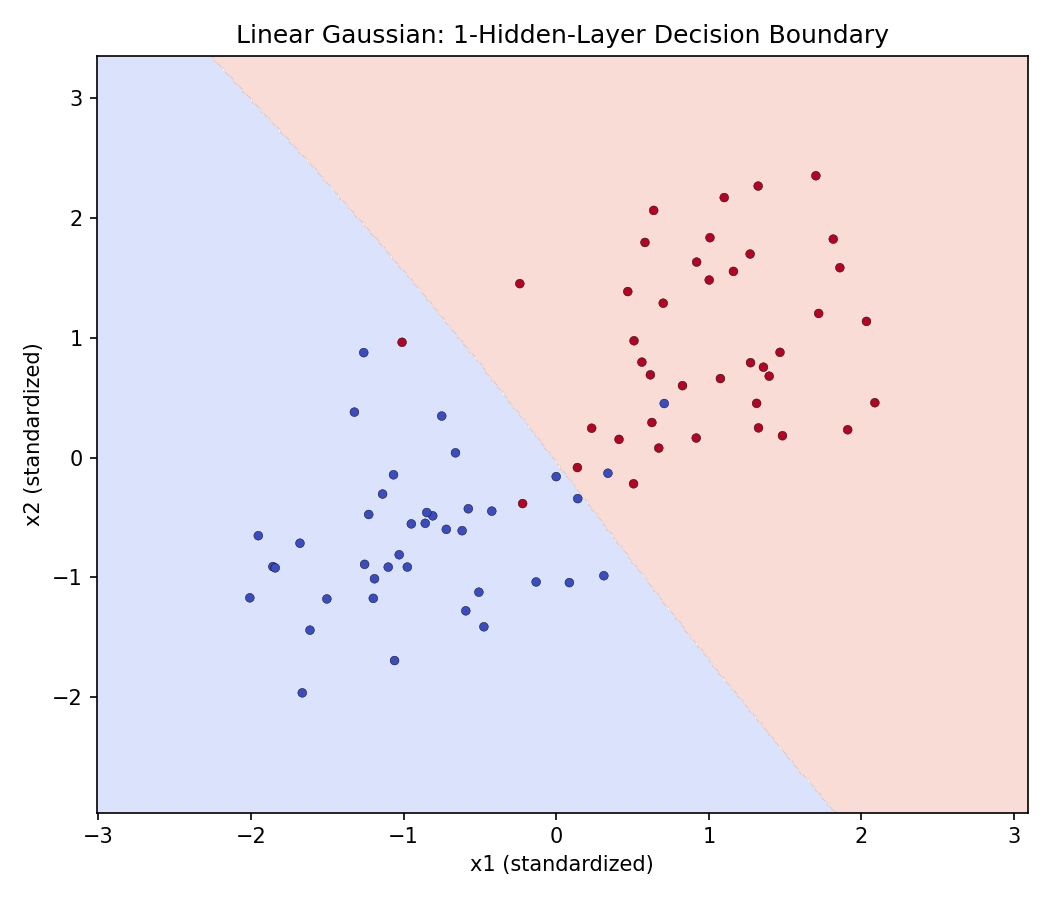
\includegraphics[width=\linewidth]{figures/linear_gaussian_hidden_layer_boundary.png}
        \caption{Linear Gaussian, hidden-layer}
    \end{subfigure}

    \vspace{0.6em}

    \begin{subfigure}{0.48\textwidth}
        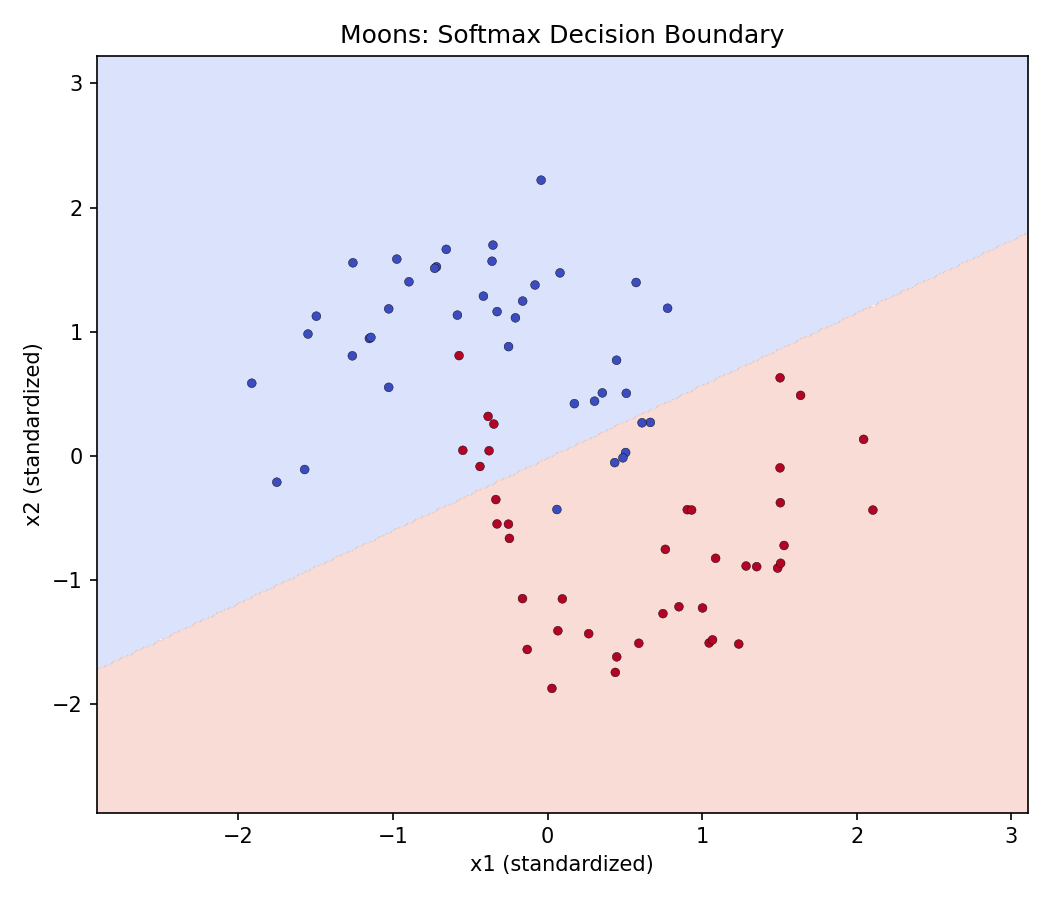
\includegraphics[width=\linewidth]{figures/moons_softmax_boundary.png}
        \caption{Moons, softmax}
    \end{subfigure}
    \hfill
    \begin{subfigure}{0.48\textwidth}
        
\includegraphics[width=\linewidth]{figures/moons_hidden_layer_boundary.png}
        \caption{Moons, hidden-layer}
    \end{subfigure}
    \caption{Decision boundaries for both datasets and both model classes.}
    \Description{Four decision-boundary plots. On linear Gaussian, softmax and hidden-layer boundaries are both nearly linear and produce similar separation. On moons, the softmax boundary is approximately linear and misses curved structure, while the hidden-layer boundary curves to follow the class geometry and separates classes more accurately.}
    \label{fig:all-boundaries}
\end{figure*}

\subsection{Digits benchmark (fixed split)}
We evaluate final selected digits configurations on the provided fixed train/validation/test split: softmax regression and one-hidden-layer network (width 32) with Adam. Selection is based on validation cross-entropy, while reporting is on held-out test data.

\begin{table}[t]
    \centering
    \caption{Digits final single-seed test results (seed 42).}
    \label{tab:digits-final}
    \begin{tabular}{lcc}
        \toprule
        Model & Test CE & Test Acc \\
        \midrule
        Softmax & 0.2710 & 0.9348 \\
        Hidden-layer (Adam) & 0.1268 & 0.9565 \\
        \bottomrule
    \end{tabular}
\end{table}

The hidden-layer model improves test cross-entropy and test accuracy over the softmax baseline on digits for the selected final setup.

\subsection{Digits repeated-seed uncertainty (n=5)}
To account for optimization stochasticity, we run the final digits configurations across five seeds (42--46) and report mean, standard deviation, and 95\% confidence intervals.

\begin{table}[t]
    \centering
    \caption{Digits repeated-seed summary (n=5).}
    \label{tab:digits-ci}
    \resizebox{\columnwidth}{!}{%
    \begin{tabular}{lcccccc}
        \toprule
        Model & Metric & Mean & Std & 95\% CI Low & 95\% CI High & n \\
        \midrule
        Softmax & Test CE & 0.2699 & 0.0014 & 0.2682 & 0.2717 & 5 \\
        Softmax & Test Acc & 0.9370 & 0.0012 & 0.9354 & 0.9385 & 5 \\
        Hidden-layer (Adam) & Test CE & 0.1655 & 0.0349 & 0.1221 & 0.2088 & 5 \\
        Hidden-layer (Adam) & Test Acc & 0.9592 & 0.0051 & 0.9529 & 0.9656 & 5 \\
        \bottomrule
    \end{tabular}%
    }
\end{table}

Across repeated seeds, the hidden-layer configuration maintains better average accuracy and lower average cross-entropy, while showing higher CE variance than softmax.

\subsection{Hidden-layer optimizer ablation on digits}
For the one-hidden-layer digits model, we compare SGD, Momentum, and Adam under the fixed protocol and report seed-42 test metrics.

\begin{table}[t]
    \centering
    \caption{Digits hidden-layer optimizer ablation (seed 42).}
    \label{tab:digits-opt-ablation}
    \begin{tabular}{lcc}
        \toprule
        Optimizer & Test CE & Test Acc \\
        \midrule
        SGD & 0.1684 & 0.9511 \\
        Momentum & 0.1505 & 0.9565 \\
        Adam & 0.1268 & 0.9565 \\
        \bottomrule
    \end{tabular}
\end{table}

Momentum and Adam tie on test accuracy here, while Adam achieves the lowest cross-entropy; therefore Adam is selected as the final hidden-layer optimizer in this report.

\section{Advanced Track}
In this section, we investigate the structural properties of the Digits dataset (d=64) through the application of Singular Value Decomposition (SVD\textbf{)}. The primary objective is to define the inherent dimensionality of the handwritten digits and evaluate the feasibility of linear compression without significant information loss.
\begin{figure}
    \centering
    
\includegraphics[width=1\linewidth]{track_a_scree.png}
    \caption{Track A Scree Plot}

        \label{fig:placeholder}
\end{figure}
By analyzing the distribution of eigenvalues, we observed that the first principal component captures approximately 15\% of the total variance. Quantitatively, the first 10 components capture roughly 75\% of the dataset’s total variance. The smooth decay of these singular values confirms that while the pixel space is 64-dimensional, the significant signal is concentrated in a much lower-dimensional linear subspace. This mathematically justifies discarding the trailing 24 dimensions, as they likely represent redundant background pixels or high-frequency noise.
\begin{figure}
        \centering
        
\includegraphics[width=1\linewidth]{track_a_viz_2d.png}
        \caption{Track A 2D Visualization}
        \label{fig:placeholder}
    \end{figure}
To visualize class separability, we projected the 64-dimensional samples onto the first two principal components (PC\_1, PC\_2). The 2D Visualization reveals that while specific digits (such as '0' and '4') form relatively isolated clusters in the periphery, there is a high degree of overlap in the central region among digits like '1', '8', and '9'. This "entanglement" provides empirical evidence that a linear hyperplane in low dimensions cannot perfectly segregate the classes, providing the experimental reasoning for utilizing non-linear hidden layers to warp the feature space into a separable configuration.

We quantified the trade-off between dimensionality (m) and model performance using a Softmax Regression classifier ($\eta=0.1, \lambda=0.01$). The results demonstrate a "plateau" effect: moving from m=10 to m=40 components recovers 99.6\% of the raw model's accuracy. This implies that the "intrinsic dimensionality" for reliable digit recognition is approximately m=40, allowing for a 37.5\% reduction in feature space with negligible performance loss.

In conclusion, this analysis demonstrates that linear dimensionality reduction effectively isolates the core "signal" of the dataset, identifying m=40 as the optimal threshold for balancing computational efficiency and classification accuracy.

\section{Discussion}
The experiments provide two clear messages. First, additional model complexity is not automatically useful. On linear Gaussian, the hidden layer does not improve test accuracy over the linear baseline, so the simpler model is already sufficient. Second, representation learning matters when geometry is nonlinear. On moons, the hidden layer transforms the feature space so the final separator fits the structure better, yielding a substantial performance gain.

These observations are consistent with the project's central framing question. The appropriate model class depends on data geometry and evidence, not on a blanket preference for nonlinear models.

\section{Limitations}
This report includes synthetic tasks, the fixed digits benchmark, repeated-seed summaries for final digits configurations, optimizer ablation for the hidden-layer digits model, and Track A (SVD/PCA) analysis. Remaining limitations are that the optimizer ablation is reported for one fixed seed and the study is restricted to the provided datasets and protocol, so conclusions should be interpreted within this capstone scope rather than as universal claims across broader data regimes.

\section*{Acknowledgments}
We thank the course instructors and teaching assistants for guidance.

\bibliographystyle{ACM-Reference-Format}
\bibliography{references}

\appendix

\section{Contribution Statement}
Agshin Fataliyev led Track A implementation and analysis (SVD/PCA workflow, scree/2D interpretation, and dimensionality comparison summary), and contributed to broader result interpretation and final report integration.

Sabuhi Nazarov led core implementation and integration across the main source files and experiment scripts, including training/evaluation pipeline updates, configuration refactoring, experiment orchestration, handled documentation maintenance and updates.

\end{document}
